%!TEX ROOT = main.tex

\chapter{Results and Discussions}

\section{Introduction}
The results of the experiments are shown in this section. The differences in the accuracy and performance of each of the methods would be discussed and analysed. Hopefully, the results and discussions would be able to answer the research questions posted in the beginning of this research.

\section{Term frequency}

\begin{table}[H]
	\centering
	\caption{Term frequency}
	\label{tbl:termFrequency}
	\begin{tabular}{|| c | c | c | c||}
		\hline
		ML & no of features & accuracy & time taken (s) \\ [0.5ex]
		\hline\hline
		kNN & 8000 & 0.31 & 3.74 \\ 
		\hline
		SVM & 8000 & 0.81 & 5.27 \\
		\hline
		NN & 8000 & 0.84 & 91.82 \\
		\hline
	\end{tabular}
\end{table}

Term frequency is one of most common feature extraction method in text. It convert all the words in the dataset into a matrix where each column is a word and the value in each of the cells are the number of times each word appear in the text. Each row in the matrix is a document. This vector space model representation of the words would result in a sparse matrix since each of the documents only contains a subset of all the words in the whole dataset. 

In this experiment, the number of features of vector space model from term frequency extraction is limited to 8000, this is because of the memory constraint of the machine, if it is unlimited, the resulting matrix would be of bigger size and would have the risk of running out of memory while processing the matrix. 

In the results shown above, \ac{nn} achieved an accuracy of 0.84 which is the best accuracy out of the 3 classification algorithms but it is also the one that takes the longest to process which is 91.82s. \Ac{knn} took the least time to process, 3.74s but has the lowest accuracy score, 0.31. Overall performance, \ac{svm} is the best, it only took 5s to process, which is 80s less than \ac{nn} and has an accuracy of 0.81 which is comparable with \ac{nn}. 

\Ac{knn} accuracy is low in this scenario is possibly due to the sparsity of the feature matrix or vector space model. The data points are few and far in between. \Ac{knn} is designed for low dimensional data therefore it doesn't perform well in large and sparse data. The underlying reason would be due to \ac{knn} classify a new data point based on the distance of the new data point with the nearby data points. Since the other data points are few and sparse, the classification of the new data points would be biased to the few data points that are near. This bias would reduce the accuracy of the classification. \cite{knnDrawback}

Neural Network (\ac{nn}) took the longest time to process the features, this is due to the number of hidden layers in \ac{nn}. The vector space model even though sparse has high dimension, \ac{nn} would need as much if not more neurons as the number of features to process the data. This processing would takes both time and computing power.

\Ac{svm} depends on the prominent features of the dataset, the support vectors to classify the dataset so it is relatively faster and as accurate.

\section{Term frequency with naive dimension reduction}

\begin{table} [h]
	\centering
	\caption{Term frequency with naive dimension reduction}
	\label{tbl:termFrequencyNaive}
	\begin{tabular}{|| c | c | c | c ||}
		\hline
		ML & no of features & accuracy & time taken (s) \\ [0.5ex]
		\hline\hline
		kNN & 6026 & 0.25 & 4.16 \\ 
		\hline
		kNN & 4058 & 0.26 & 4.22 \\ 
		\hline
		kNN & 2020 & 0.27 & 4.52 \\ 
		\hline
		kNN & 1030 & 0.30 & 5.08 \\ 
		\hline
		kNN & 508 & 0.32 & 5.14 \\ 
		\hline
		kNN & 108 & 0.30 & 5.10 \\ 
		\hline
		kNN & 54 & 0.26 & 4.77 \\ 
		\hline\hline
		SVM & 6026 & 0.81 & 6.57 \\
		\hline
		SVM & 4058 & 0.76 & 6.63 \\
		\hline
		SVM & 2020 & 0.74 & 7.85 \\
		\hline
		SVM & 1030 & 0.68 & 9.52 \\
		\hline
		SVM & 508 & 0.64 & 20.86 \\
		\hline
		SVM & 108 & 0.42 & 37.48 \\
		\hline
		SVM & 54 & 0.31 & 39.71 \\
		\hline\hline
		NN & 6026 & 0.85 & 67.65 \\
		\hline
		NN & 4058 & 0.83 & 63.72 \\
		\hline
		NN & 2020 & 0.78 & 43.38 \\
		\hline
		NN & 1030 & 0.73 & 42.89 \\
		\hline
		NN & 508 & 0.65 & 50.37 \\
		\hline
		NN & 108 & 0.41 & 82.84 \\
		\hline
		NN & 54 & 0.34 & 82.39 \\
		\hline
	\end{tabular}
\end{table}

The feature extraction method used in this experiment is same as the experiment above but dimension reduction method is applied to the resulting matrix before training. The dimension reduction algorithm used in this experiment is a naive one which means that the columns with the least occurrence of word are removed assuming those words are unimportant and would not have much influence on the accuracy.

In this experiment, \ac{knn} still has the worst performance among the 3 which is at 0.25 with 6026 number of features. As the number of features decreases to 508, the accuracy increases slightly to 0.32. As the number of features decreases, the time taken for \ac{knn} to produce the result increases from 4.16s to 4.77s.

\Ac{svm} and \ac{nn} have the same trend in this experiment, the accuracy decreases as the number of features decreases. Accuracy of \ac{svm} decreases from 0.81 to 0.31 as the number of features decreases from 6026 to 54. The time taken by \ac{svm} increases as the amount of features decreases, it increases from 6.57s to 39.71s.

The time taken by \ac{svm} increases quite drastically when the number of features decreased. Since the dimension reduction method used is a naive dimension reduction, no high computational cost functions are involved, the reduction would not take much time. The bulk of the time taken is for \ac{svm} to classify the text. The number of features in the matrix decreases thus the sparsity of the vector space model decreases, resulting in a denser vector space model. In this case, \ac{svm} need to take into account more data points to calculate an optimum hyperplane to separate the data points into different classes. Therefore, more time is taken to compute the optimum hyperplane.

On the other hand, the accuracy of \ac{nn} decreases from 0.85 to 0.34 as the number of features decreases from 6026 to 54. However, the time taken by NN fluctuates from 67.65s to 42.29s and then to 82.39s when the amount of features decreases from 6026 to 1030 then to 54. The overall decrement in time taken is possibly due to the reduction of features, less neurons are needed to process the data and thus the speedup.

\Ac{svm} and \ac{nn} performs better when there are more features, the time taken would be relatively lesser and the accuracy would be higher than in the scenarios with lesser number of features. This show that these 2 classification algorithms are able to process features in a large and sparse vector space effectively.

\subsection{Graph of Term Frequency with Naive Dimension Reduction}
\begin{figure} [H]
	\centering
	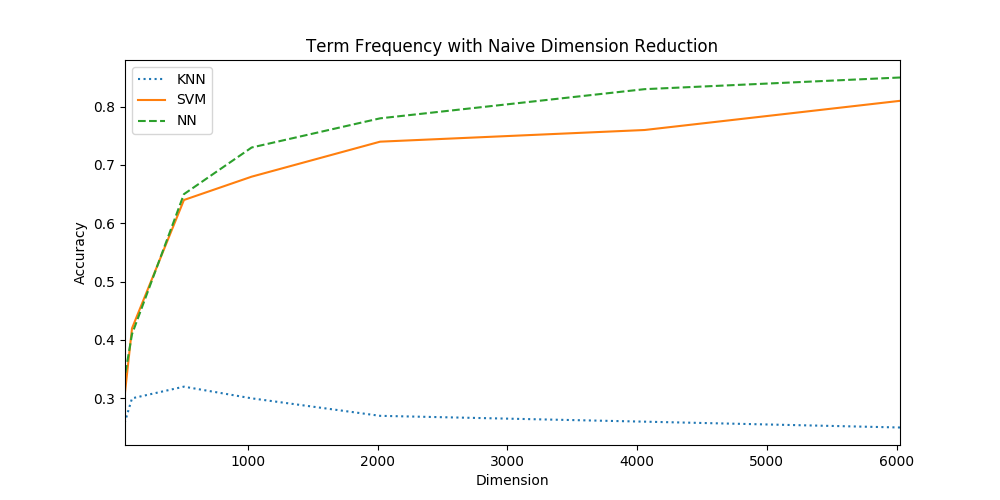
\includegraphics[width=\textwidth]{tfnaive}
	\caption{Term Frequency with Naive Dimension Reduction}
	\label{fig:tfnaive}
\end{figure}

The figure above illustrates more clearly the results shown in this section. The graph shows the change in accuracy of the classification models as the number of features decreases.

In this graph, it is clearly shown that \ac{knn} is not as efficient as \ac{svm} and \ac{nn}, its accuracy is much lower than that of \ac{svm} and \ac{nn} across the spectrum of dimension. The accuracy of \ac{knn} increases slightly as the number of features decreases.

\Ac{nn} has a slightly higher accuracy than \ac{svm} all the scenarios when the number of features is greater than 1000. When the number of features is lesser than 1000, both \ac{nn} and \ac{svm} has similar performance. The accuracy of these classification models decreases as the number of features decreases, which is expected. When the number of features decreases, the classification models would have less information to classify a document, thus the result is more error prone.\\

\section{Term frequency with truncated SVD}

\begin{table} [H]
	\centering
	\caption{Term frequency with truncated SVD}
	\label{tbl:termFrequencySvd}
	\begin{tabular}{|| c | c | c | c||}
		\hline
		ML & no of features & accuracy & time taken (s) \\ [0.5ex]
		\hline\hline
		kNN & 6026 & 0.29 & 809.33 \\
		\hline
		kNN & 4058 & 0.31 & 489.86 \\ 
		\hline
		kNN & 2020 & 0.39 & 222.31 \\ 
		\hline
		kNN & 1030 & 0.45 & 112.66 \\ 
		\hline
		kNN & 508 & 0.48 & 58.00 \\ 
		\hline
		kNN & 108 & 0.55 & 15.52 \\ 
		\hline
		kNN & 54 & 0.53 & 7.76 \\ 
		\hline\hline
		SVM & 6026 & 0.81 & 669.01 \\
		\hline
		SVM & 4058 & 0.79 & 391.88 \\
		\hline
		SVM & 2020 & 0.79 & 165.82 \\
		\hline
		SVM & 1030 & 0.78 & 93.1 \\
		\hline
		SVM & 508 & 0.77 & 78.48 \\
		\hline
		SVM & 108 & 0.65 & 54.03 \\
		\hline
		SVM & 54 & 0.57 & 41.11 \\
		\hline\hline
		NN & 6026 & 0.81 & 370.22 \\
		\hline
		NN & 4058 & 0.80 & 213.13 \\
		\hline
		NN & 2020 & 0.79 & 82.52 \\
		\hline
		NN & 1030 & 0.79 & 54.10 \\
		\hline
		NN & 508 & 0.77 & 35.85 \\
		\hline
		NN & 108 & 0.69 & 25.51 \\
		\hline
		NN & 54 & 0.64 & 23.01 \\
		\hline
	\end{tabular}
\end{table}

In this experiment, the feature extraction or document representation method used is still term frequency but the dimension reduction algorithm has changed. Instead of reducing the dimension of the feature matrix naively by removing the terms that has the lowest frequency, truncated \ac{svd} is used. Truncated \ac{svd} would reduce the dimension of the vector space model by retrieving the features with maximum variance in the data.

The number of features shown in the table above is the number of columns in the resulting matrix after truncated \ac{svd} is applied.

Similar with the trend in the previous experiment (term frequency with naive dimension reduction), the accuracy of \ac{knn} increases slightly, from 0.29 to 0.55 when the features decreases from 6026 to 108, but the resulting accuracy is still far from satisfactory. The time taken by \ac{knn} decreases from 809.33s to 7.76s as the number of features decreases. The trend of accuracy increment as the number of features decrease cease when the number of features is reduced to 54. \Ac{knn} accuracy decrease from 0.55 to 0.53 at that point. The fluctuation of the accuracy would be due to \ac{knn} dependency on Euclidean distance between the data points to classify a new data. As the amount of features decrease, the feature matrix becomes less sparse, \ac{knn} would need to process less data points thus the speedup. A less sparse matrix resulting from the decrement of features also make \ac{knn} classification more accurate and less biased but when the features decrease to an extent where there is no sufficient data to classify a data point correctly, the accuracy dropped.

The accuracy of \ac{svm} and \ac{nn} also have the same trend with the previous experiment, the accuracy decreases slightly when the number of features decreases. Accuracy of \ac{svm} decreases from 0.81 to 0.57 and the accuracy of \ac{nn} decreases from 0.81 to 0.64 as the number of features decreases from 6026 to 54.

As expected, the time taken by the classification model to reduce the dimension and predict the result decreases as the number of features decreases. However, when compare with previous experiments, the time taken in this experiment is astoundingly higher in the case where the features amount to 6026. \Ac{svd} would be the culprit, dimension reduction comes at a cost which is processing power. To calculate the maximum variance of the features and transform the feature matrix into a smaller dimension would require no small feats of calculation, this would consume both time and processing power.

However, the resulting accuracy is not as good as the experiment with term frequency without any dimension reduction. This is expected because the number of features decreased, the classification would have lesser information to classify a new document correctly. Therefore, it is shown that the reduction in features could reduce the memory space needed to store the feature matrix but it came at the cost of more processing power, longer processing time and most importantly a less accurate result.


Comparing the performance of the classification models in this experiment with the second experiment, term frequency with naive dimension reduction, the performance of the classification models are slightly better with \ac{svd}. All the 3 classification models has a slightly higher accuracy across the dimension size when compare with the results of the second experiment. This shows the advantage of \ac{svd} over naive dimension reduction. \Ac{svd} transformed the feature matrix into smaller dimension but retaining the maximum variance or the most prominent feature of the data. Therefore, models trained with \ac{svd} should have a better performance than those that trained with naive dimension reduction.

This experiment shows that SVD is a better dimension reduction algorithm than naive dimension reduction method. In this and the previous two experiments, term frequency is applied, it might be too simplistic and the features obtain are not optimum. The next experiments would apply a different document representation algorithm to investigate further the effect of dimension reduction has on classification model performance and compare the performance of different document representation method.\\

\subsection{Graph of Term Frequency with SVD}
\begin{figure} [H]
	\centering
	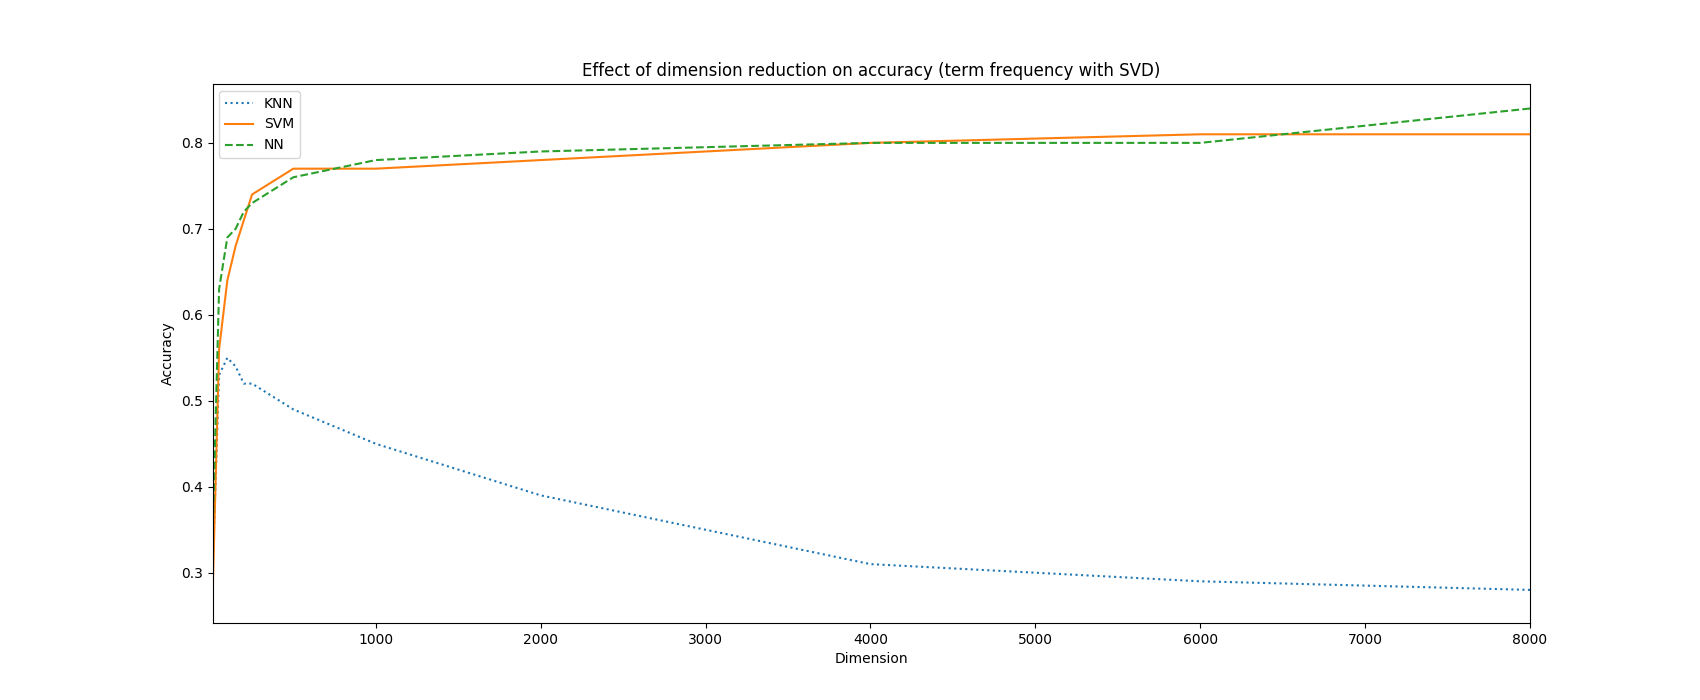
\includegraphics[width=\textwidth]{tfsvd}
	\caption{Term Frequency with SVD}
	\label{fig:tfsvd}
\end{figure}

The figure illustrates what have been described above. This graph show the advantage of SVD has over naive dimension reduction. The accuracy of \ac{knn} increases further when the dimension decreases when compare to the experiment of term frequency with naive dimension reduction. At the extreme point, \ac{knn} has an accuracy of 0.53 while in the previous experiment, \ac{knn} achieve a meager 0.26 with same number of features.

The accuracy of \ac{svm} and \ac{nn} are more stable when SVD is applied. The accuracy of both classification models does not decrease as much when the dimension decreases. Even at the extreme decrement, the accuracy achieved is better.

By comparing the result of these 2 experiments, it is seems that SVD is a better dimension reduction method. The next few experiments would explore another document representation method and determine which of the document representation methods is more efficient and optimised in extracting features from news articles.\\

\section{TF-IDF}
\begin{table} [H]
	\centering
	\caption{TF-IDF}
	\label{tbl:tfidf}
	\begin{tabular}{|| c | c | c | c||}
		\hline
		ML & no of features & accuracy & time taken (s) \\ [0.5ex]
		\hline\hline
		kNN & 8000 & 0.76 & 3.71 \\ 
		\hline
		SVM & 8000 & 0.87 & 2.39 \\
		\hline
		NN & 8000 & 0.88 & 55.82 \\
		\hline
	\end{tabular}
\end{table}

The previous experiments found that \ac{svd} has a slight edge over naive dimension reduction. In this and the next experiments, the effect on dimension reduction is further explored. The performance of the classification models in the previous experiments might be limited by the document representation method used, namely term frequency. It is a simple algorithm and the vector space model generated may not contain enough prominent features for the classification models to classify the documents accurately. Therefore, in this and the next few experiments, a different document representation method is used.
 
The document representation algorithm applied in this experiment is \ac{tfidf}. In contrast with term frequency which only take the frequency of each word into account, \ac{tfidf} takes both the frequency of each word and its rarity into account. If a term or word appear in high frequency but in many documents, this word may not be of importance and consequently is not a meaningful feature. If a word appear rarely and only in a few documents, this word would have high importance and would be a meaningful feature of the few documents.

With \ac{tfidf}, \ac{knn} can achieved a satisfactory accuracy score of 0.76 even though the number of features in the resulting matrix of \ac{tfidf} is the same with term frequency which is 8000. The vector space model of \ac{tfidf} would not be as sparse as that of term frequency which is more suitable for \ac{knn}.

\Ac{nn} is still provide the highest accuracy score of 0.88 but the time taken also the longest at 55.82s.
\Ac{nn} take the longest time to compute the result in most of the scenarios. This would be due to the number of hidden layers and the number of neurons in the \ac{nn}. In the experiments, the \ac{nn} applied has at least 1 hidden layer and the hidden layers would consist of 100 neutrons. Each of these neutron is a processing unit to compute the input feature. Due to the large size of the hidden layer and large size of the feature matrix, \ac{nn} would take a long time to feed each of the feature through the hidden layers and each of the neutron. The structure of \ac{nn} caused the long time taken, unless special hardware such as graphic processors or higher power processor is used, the time taken by \ac{nn} would be higher than other classification models.

\Ac{svm} achieved an accuracy of 0.87 which is just 0.01 shy of what achieved by \ac{nn} and the time taken is the lowest among the 3 which is 2.39s. \Ac{svm} can achieve high accuracy even with high dimension data, because \ac{svm} uses the prominent features or support vectors from the data to perform classification, \ac{svm}'s computational complexity is independent of the dimension of the data. \cite{dimRedCat}.

In comparison with the first experiment that apply term frequency document representation without dimension reduction, the performance of the classification models significantly improve. \Ac{knn} accuracy has more than doubled from 0.31 to 0.76. \Ac{svm} accuracy increases from 0.81 to 0.87 while accuracy of \ac{nn} increases from  0.84 to 0.88. Besides accuracy, the time taken also improved, time taken by \ac{svm} reduces from 5.27s to 2.39s while time taken by \ac{nn} reduces from 91.82s to 55.82s. All these improvements are achieved with the same number of features in the vector space, which is 8000. 

The performance of the classification models in this experiment is also better than those in the 2 experiments above with dimension reduction. However this may not be a fair comparison because the different number of features are used and dimension reductions are not applied in this experiment. Dimension reduction algorithms would be applied to the vector space model from \ac{tfidf} in the following experiments in order to have a fair comparison.

The performance increment from term frequency to \ac{tfidf} seems to prove that \ac{tfidf} is a better document representation method and more optimised to extract features from news articles.\\

\section{TF-IDF with naive dimension reduction}

\begin{table} [ht]
	\centering
	\caption{TF-IDF with naive dimension reduction}
	\label{tbl:tfidfNaive}
	\begin{tabular}{|| c | c | c | c||}
		\hline
		ML & no of features & accuracy & time taken (s) \\ [0.5ex]
		\hline\hline
		kNN & 6026 & 0.76 & 3.76 \\ 
		\hline
		kNN & 4058 & 0.74 & 3.89 \\ 
		\hline
		kNN & 2020 & 0.69 & 4.00 \\ 
		\hline
		kNN & 1030 & 0.59 & 4.35 \\ 
		\hline
		kNN & 508 & 0.49 & 4.98 \\ 
		\hline
		kNN & 108 & 0.08 & 12.28 \\ 
		\hline
		kNN & 54 & 0.06 & 21.20 \\ 
		\hline\hline
		SVM & 6026 & 0.87 & 2.49 \\
		\hline
		SVM & 4058 & 0.85 & 2.45 \\
		\hline
		SVM & 2020 & 0.82 & 2.50 \\
		\hline
		SVM & 1030 & 0.75 & 2.64 \\
		\hline
		SVM & 508 & 0.68 & 2.98 \\
		\hline
		SVM & 108 & 0.41 & 4.43 \\
		\hline
		SVM & 54 & 0.32 & 11.63 \\
		\hline\hline
		NN & 6026 & 0.87 & 48.32 \\
		\hline
		NN & 4058 & 0.85 & 42.75 \\
		\hline
		NN & 2020 & 0.81 & 37.77 \\
		\hline
		NN & 1030 & 0.74 & 48.2 \\
		\hline
		NN & 508 & 0.65 & 80.45 \\
		\hline
		NN & 108 & 0.45 & 76.17 \\
		\hline
		NN & 54 & 0.35 & 73.92 \\
		\hline
	\end{tabular}
\end{table}

Similar with the experiment with term frequency, naive dimension reduction is applied to the vector space model generated from \ac{tfidf}. The trend over all the 3 machine learning models when the number of features decreases are similar. The accuracy of the classification models decreases and the time taken increases. 

The accuracy achieved by \ac{knn} with \ac{tfidf} plus naive dimension reduction is still passable at 0.76 when the features reduced from 8000 to 6026. \Ac{knn}'s accuracy dropped slightly to 0.69 when the number of features decreases to 20200. When the number of features decreases from 2020 to 54, the accuracy of \ac{knn} dropped for quite a large margin, from 0.69 to 0.06. The time taken by \ac{knn} increases from 3.76s to 21.20s as the features decreases.

\Ac{svm} has the same behaviour with \ac{knn} in this experiment, its accuracy decreases from 0.87 to 0.75 and then to 0.32 when the number of features decreases from 6026 to 1030 to 54. The time taken increases from 2.49s to 11.63s as the number of features decreases.

\Ac{nn} also has the similar trend in accuracy as the number of features decreases. \Ac{nn}'s accuracy decreases from 0.87 to 0.74 when the number of features decreases from 6026 to 1030. The time taken increases from 48.32s to 73.92s.

In the scenarios where the number of features are almost halved, from 8000 to 4058, the performance of the classification models are still comparable with the performance achieved with just \ac{tfidf} without any dimension reduction. The accuracy are almost the same, the time taken is similar except \ac{nn} which has quite a speedup when the number of features is reduced to 4058. This might a sweet spot between dimension reduction and accuracy. At this point, the accuracy is still satisfactory and the time taken is lesser. If \ac{nn} and dimension reduction is applied in the real world, the dimension of the news articles would have to be at this level. At this level, the classification model is best positioned to reap the reward of dimension reduction, less memory to store the feature matrix, less time is used to compute the result and a comparable accuracy is achieved.

It can be deduced that with naive dimension reduction, the number of features and memory needed to store the vector space model is reduced. With this reduced number of features, the classification models can still achieve comparable performance at a slightly decreased capacity.

The slight reduction in performance is mainly because of the reduction in dimension. As the amount of information became lesser, less information is available to train a comprehensive model. Therefore, the accuracy of the models decrease. Even though the dimension reduction applied is a naive one and less computing intensive, it still increases the time taken compared with just with \ac{tfidf}. The more reduction is performed, the time taken would increase as well.

\subsection{Graph of TF-IDF with Naive Dimension Reduction}
\begin{figure} [H]
	\centering
	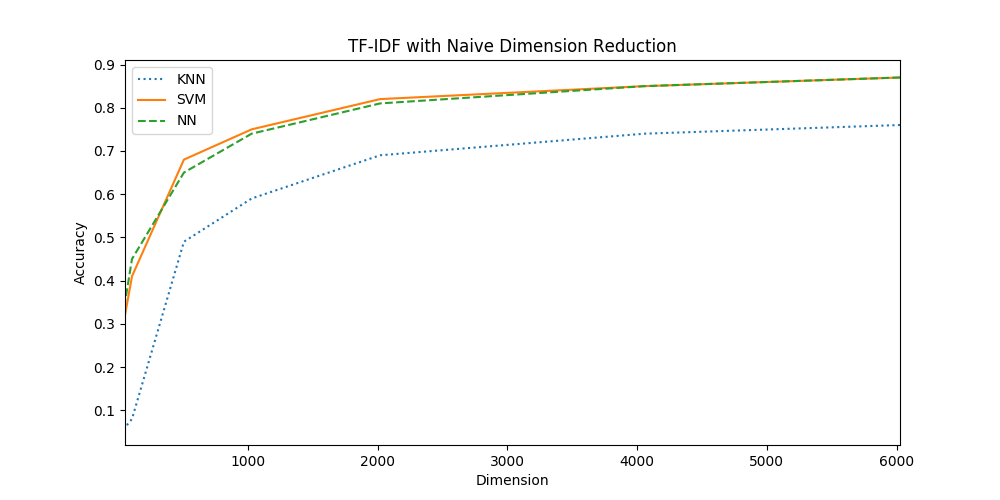
\includegraphics[width=\textwidth]{tfidfnaive}
	\caption{TFIDF with Naive Dimension Reduction}
	\label{fig:tfidfnaive}
\end{figure}

The graph above illustrates the results of this experiments. All three classification models have the same decreasing trend in their accuracy as the dimension decreases. 

\Ac{svm} and \ac{nn} have similar performance with each other. \Ac{knn} performs much better with tfidf than with term frequency document representation method but its accuracy is still lesser than that of \ac{svm} and \ac{nn}.

\section{TF-IDF with truncated SVD}

\begin{table} [h]
	\centering
	\caption{TF-IDF with truncated SVD}
	\label{tbl:tfidfSvd}
	\begin{tabular}{|| c | c | c | c||}
		\hline
		ML & no of features & accuracy & time taken (s) \\ [0.5ex]
		\hline\hline
		kNN & 6026 & 0.77 & 833.65 \\
		\hline
		kNN & 4058 & 0.77 & 487.82 \\ 
		\hline
		kNN & 2020 & 0.58 & 221.26 \\ 
		\hline
		kNN & 1030 & 0.56 & 111.36 \\
		\hline
		kNN & 508 & 0.54 & 57.40 \\ 
		\hline
		kNN & 108 & 0.69 & 15.48 \\ 
		\hline
		kNN & 54 & 0.70 & 8.04 \\ 
		\hline\hline
		SVM & 6026 & 0.87 & 374.90 \\
		\hline
		SVM & 4058 & 0.87 & 194.99 \\
		\hline
		SVM & 2020 & 0.86 & 72.16 \\
		\hline
		SVM & 1030 & 0.85 & 35.19 \\
		\hline
		SVM & 508 & 0.83 & 18.41 \\
		\hline
		SVM & 108 & 0.77 & 6.40 \\
		\hline
		SVM & 54 & 0.74 & 4.68 \\
		\hline\hline
		NN & 6026 & 0.86 & 384.91 \\
		\hline
		NN & 4058 & 0.86 & 203.26 \\
		\hline
		NN & 2020 & 0.84 & 86.47 \\
		\hline
		NN & 1030 & 0.82 & 52.29 \\
		\hline
		NN & 508 & 0.81 & 46.11 \\
		\hline
		NN & 108 & 0.79 & 27.63 \\
		\hline
		NN & 54 & 0.78 & 25.36 \\
		\hline
	\end{tabular}
\end{table}

In this last experiment, truncated \ac{svd} dimension reduction is applied to the resulting vector space model from \ac{tfidf}. Similar with experiment before, each of the classification models would be tested with several set of vector space model, each with different number of features. To put it in perspective, the number of features without reduction is 8000. 

When the number of features are at 4058 which is about halved, \ac{knn} still can produced an accuracy of 0.77 which is similar with what is achieved with \ac{tfidf} without dimension reduction. The same goes to \ac{svm} and \ac{nn}, at 4058 features, the accuracy are quite similar with \ac{tfidf} without dimension reduction. However, when the dimension of the vector space model is reduced to 2020, the accuracy across the 3 classification models dropped. \Ac{knn} being the most drastic, its accuracy dropped to 0.58 while \ac{svm} and \ac{nn} dropped to 0.86 and 0.84 respectively, which is slightly worse than before but it is still satisfactory.

Comparing with the results of the experiment with \ac{tfidf} and naive dimension reduction, this performance of the classification models with truncated \ac{svd} has a slight advantage. The accuracy is slightly better with truncated \ac{svd} than that with naive dimension reduction. This would be due to the advantage of truncated \ac{svd} obtaining the maximum variance of the features over naive dimension reduction.

The time taken in this experiment is much higher than the experiment of \ac{tfidf} without dimension reduction and \ac{tfidf} with naive dimension reduction, which is expected. This would be due to \ac{svd} reduction takes more time, as more calculations are needed to transform the data. However, the time taken decreased when further reduction is done, \ac{knn} take 833.65s to reduce the vector space model from 8000 to 6026 but just 8s to reduce the vector space model from 8000 to 54. Keep in mind that the time recorded here includes the time taken for the classification model to predict the test set as well as the dimension reduction time. This trend appear in \ac{svm} and \ac{nn} as well. \Ac{svm} took 374.90s to reduce 8000 to 6026 but just 4.64s to reduce 8000 to 54 while \ac{nn} took 384.91s to reduce 8000 to 6026 and 25.36s to reduce 8000 to 54. 

The decrement in time could be due to SVD reduced the features and only return the most prominent features of the news articles. These prominent features would make the differences between the categories of news articles more obvious to the classification models. Thus, the time taken to process the features is also reduced, a speedup. This speedup comes at a cost which is accuracy. For \ac{svm} and \ac{nn}, the reduction in accuracy is slight thus it would be logical to trade the slight accuracy with the speedup but in \ac{knn}, the trade off would be lopsided in the favour of time taken.\\

\subsection{Graph of TF-IDF with SVD}
\begin{figure} [ht]
	\centering
	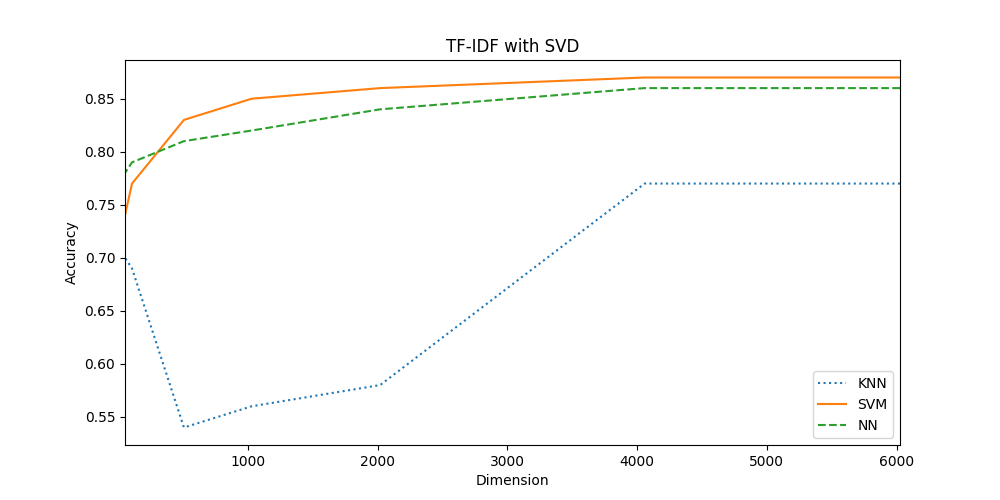
\includegraphics[width=\textwidth]{tfidfsvd}
	\caption{TFIDF with SVD}
	\label{fig:tfidfSVD}
\end{figure}

This figure show the fluctuations of the accuracy of the classification models as the dimension decreases. The feature extraction method used here is \ac{tfidf} and the dimension reduction algorithm used is truncated \ac{svd}.

\Ac{knn} accuracy remain stable at around 0.77 as the dimension decrease from 8000 to around 4000. After 4000, further decrement in dimension resulting in a decrease in accuracy. The accuracy of \ac{knn} deflected and increase from 0.54 to 0.70 when the dimension reduce from 508 to 54.

Similar to previous result, \ac{svm} and \ac{nn} accuracy remain stable around 0.8 as the dimension reduces from 8000 to 508. When the dimension of the feature matrix is reduced to an extreme of 54 then the accuracy of both \ac{svm} and \ac{nn} deteriorated to around 0.7.

\Ac{svm} is the best classification model out of the 3, it has slightly better performance than \ac{nn} in most of the scenarios. It is most resilient to the changes in dimension. This is because \ac{svm} depend on the prominent features of the data to classify the data into different classes, the dimension of the data do not has much influence on \ac{svm} computational complexity. \cite{dimRedCat}. \Ac{nn} has comparable accuracy with \ac{svm} but it would take longer time than \ac{svm} to produce the similar result.


\section{Conclusion}
From the results of the 6 experiments above, it is found that \ac{tfidf} is a better document representation algorithm than term frequency. The resulting vector space model from \ac{tfidf} can achieve a higher accuracy than that of term frequency. 

The effect of dimension reduction on the accuracy of the classification models is analysed. Dimension reduction, naive and truncated \ac{svd}, do reduce the dimension of the vector space model, reducing the memory needed to store the matrix. However, this reduction in features and information would result in a loss of accuracy. truncated \ac{svd} would be the better dimension reduction algorithm compared to the naive method because the accuracy achieved with truncated \ac{svd} is higher than that of the naive method.

Among the 3 classification models tested in the experiments, \ac{svm} is the most efficient and versatile. \Ac{svm} can achieve high accuracy (> 0.80) in most scenarios. \Ac{nn} can also achieve high accuracy in most of the cases tested but \ac{nn} is more time consuming. \Ac{svm} has an advantage over \ac{nn} on the aspect of processing time. Therefore, \ac{svm} would be the most efficient text classification model among the 3 classification models.

